% !TeX program = pdflatex
% Template modulaire FR pour CV — deux colonnes, personnalisable via commandes en tête

\documentclass[11pt, a4paper]{article}

% ===== ENCODAGE & LANGUE =====
\usepackage[T1]{fontenc}
\usepackage[utf8]{inputenc}
\usepackage{cmap} % IMPORTANT : copie PDF + compatibilité ATS
\usepackage[french]{babel}

% ===== POLICE =====
\usepackage{helvet}
\renewcommand{\familydefault}{\sfdefault}


% ===== MISE EN PAGE =====
\usepackage[left=2mm, right=2mm, top=2mm, bottom=2mm]{geometry}
\usepackage{graphicx}
\usepackage{xcolor}
\usepackage{setspace}
\usepackage{microtype}
\microtypesetup{protrusion=true, expansion=false}

\hyphenpenalty=10000
\exhyphenpenalty=10000

\linespread{1.0}

\definecolor{cvblue}{HTML}{304263}
\definecolor{cvgold}{HTML}{FFC600}

\usepackage[draft]{hyperref}
\usepackage{fancyhdr}

% --- Personnalisation ---
\newcommand{\cvname}{<<CVNAME>>}
\newcommand{\cvaddress}{<<CVADDRESS>>}
\newcommand{\cvmail}{<<CVMAIL>>}
\newcommand{\cvphone}{<<CVPHONE>>}
\newcommand{\cvlinkedin}{<<CVLINKEDIN>>}
\newcommand{\cvgithub}{<<CVGITHUB>>}
\newcommand{\jobtype}{<<JOBTYPE>>}
\newcommand{\presentation}{<<PRESENTATION>>}

% ----- COMMANDES DE MISE EN FORME -----
\newlength{\headleftwidth}
\newcommand{\headleft}[1]{%
    \vspace*{1.5ex}%
    \settowidth{\headleftwidth}{\textsc{\textbf{#1}}}%
    {\color{cvgold}\textsc{\textbf{#1}}}\par%
    \vspace*{-1.5ex}%
    {\color{cvgold}\rule{\headleftwidth}{0.4pt}}%
    \par\vspace*{0.3ex}
}

\newcommand{\headright}[1]{%
  \vspace*{1.5ex}%
  \textsc{\large\color{cvblue}#1}\par%
  \vspace*{-1.5ex}%
  {\color{cvblue}\rule{\headleftwidth}{0.4pt}}%
  \par\vspace*{0.1ex}
}

\newcommand{\dates}[1]{\hfill\mbox{\textbf{#1}}}
\newcommand{\is}{\par\vskip.5ex plus .4ex}
\newcommand{\smaller}[1]{{\small$\diamond$\ #1}}

\begin{document}

\setlength{\topskip}{0pt}
\setlength{\parindent}{0pt}
\setlength{\parskip}{0pt}
\setlength{\fboxsep}{0pt}
\raggedbottom

% ===== COLONNE GAUCHE =====
\begin{minipage}[t][\textheight]{0.30\textwidth}
  \colorbox{cvblue!90}{\color{white}
    \kern0.02\textwidth\relax
    \begin{minipage}[t][\textheight][t]{0.96\textwidth}
      \raggedright

      \vspace*{0ex}
      %\input{sections/intitule_poste.tex}

      \vspace*{2ex}
      \input{sections/disponibilite.tex}

      \vspace*{4ex}
      \input{sections/atouts.tex}

      \vspace*{4ex}
      \input{sections/langues.tex}

      \vspace*{4ex}
      \input{sections/centre_interet.tex}

      \vspace*{10ex}
      \null\hfill
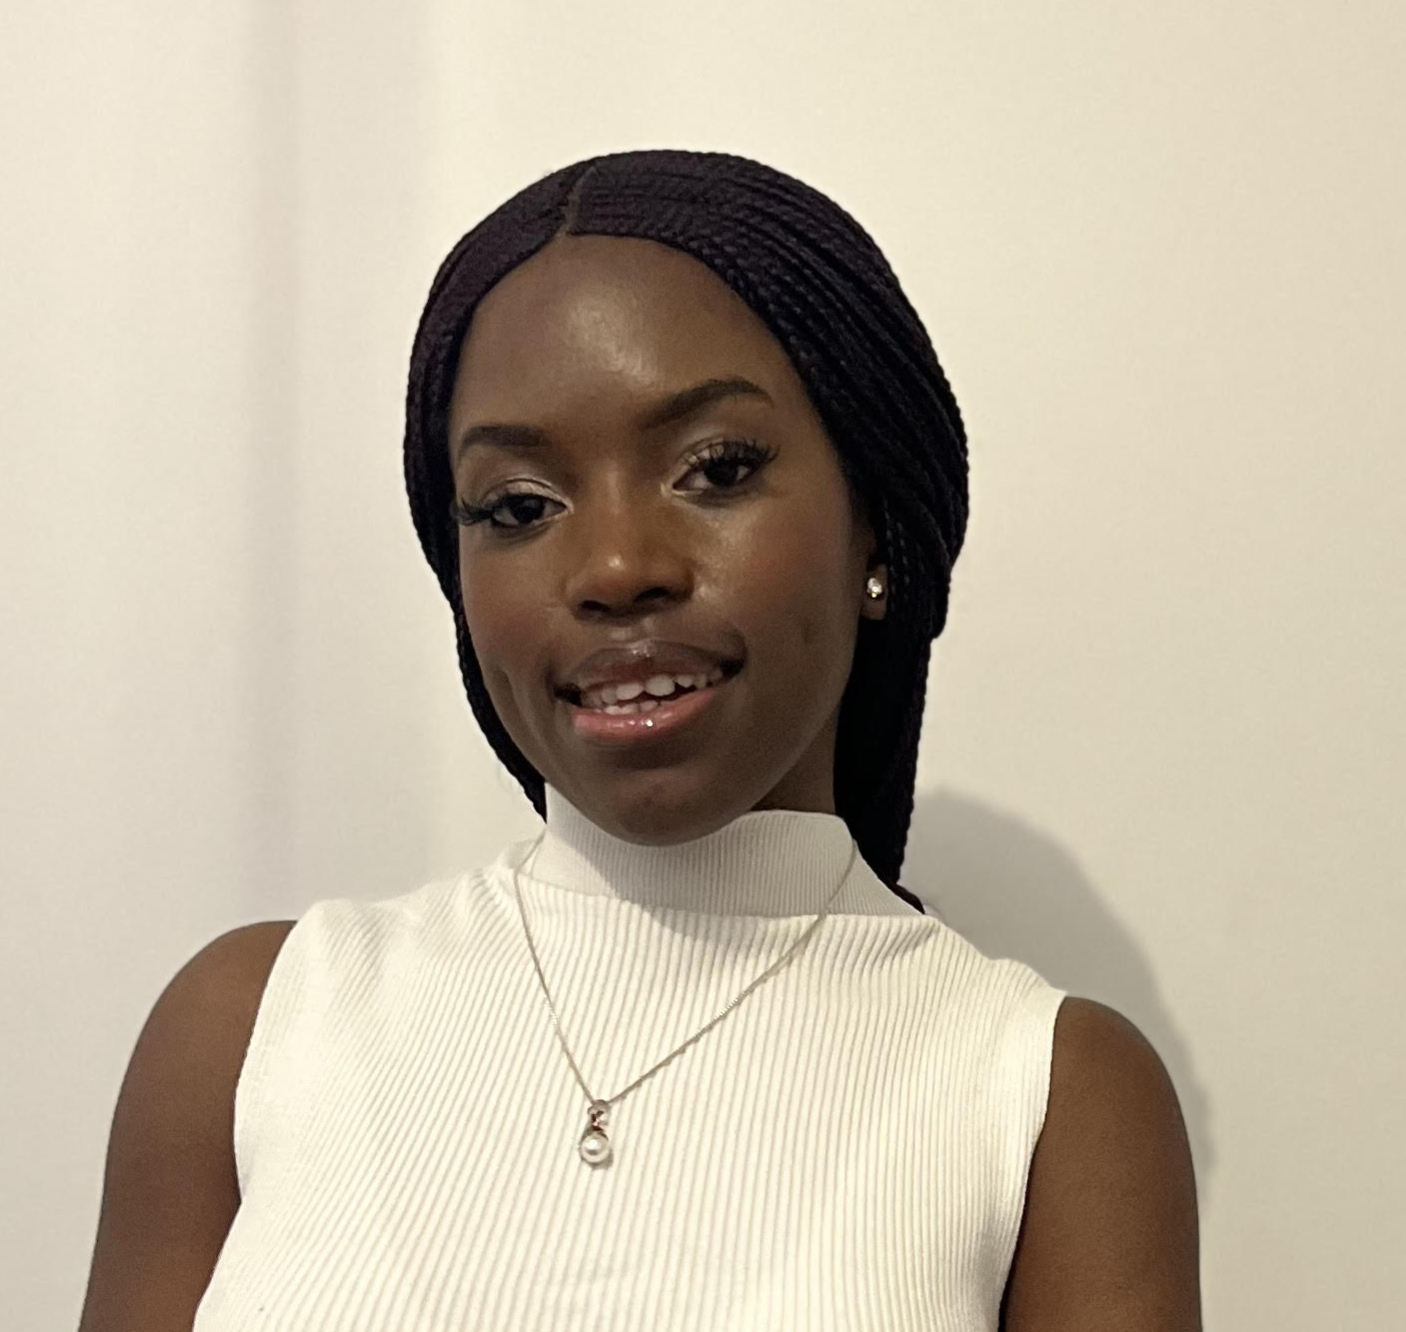
\includegraphics[width=0.65\textwidth]{../pictures/photo_cv.jpg}
\hfill\null
\vspace*{0.5ex}


      % Header: utilise les commandes definies dans main.tex
\begin{center}
    {\Large \textbf{\cvname}}\\[3pt]
    {\small \cvaddress{} \quad$\cdot$\quad \href{mailto:\cvmail}{\cvmail} \quad$\cdot$\quad
    Tél : \cvphone}\\[3pt]
    \href{https://linkedin.com/in/\cvlinkedin}{\faLinkedinIn\ \cvlinkedin} \quad$\cdot$\quad
    \href{https://github.com/\cvgithub}{\faGithub\ \cvgithub}
\end{center}

\vspace{0.2cm}


      \vspace*{10ex}
      \input{sections/informations.tex}

      \vspace*{0.1ex}

    \end{minipage}
    \kern0.02\textwidth\relax
  }
\end{minipage}%
% ===== COLONNE DROITE =====
\hskip0.01\textwidth
\begin{minipage}[t][\textheight]{0.68\textwidth}

  \setlength{\parskip}{0.1ex}
  %\vspace{0ex}

  % Exemples d'entrées — remplacez par vos expériences réelles
\textbf{Alternant Data Analyst – NaTran France (Spécialiste national des données gazières)} \hfill \textit{Septembre 2023 – Présent}\\
\textit{Ingénierie de la données, Département Data}
\begin{itemize}
    \item Développement de tableaux de bord nationaux sous \textbf{Power BI}, intégrant des jeux de données hétérogènes et réduisant le temps de reporting de 40\%.
    \item Conception et optimisation de pipelines de traitement de données avec \textbf{Python (Pandas, PySpark)}, automatisant des tâches récurrentes.
\end{itemize}

% Ajoutez d'autres expériences au besoin

  \vspace*{5ex}

  \input{sections/projets.tex}
  \vspace*{5ex}

  \input{sections/competences_techniques.tex}
  \vspace*{5ex}

  \input{sections/formations.tex}
  \vspace*{5ex}

  % Certifications — listez vos certifications ici
\begin{itemize}
    \item Microsoft Certified: Data Analyst Associate (en cours) – Power BI
    \item Bloomberg Market Concepts (BMC) (en cours)
    \item Certification AMF (en cours)
\end{itemize}


\end{minipage}

\end{document}